\documentclass[paper=letterpaper,fontsize=11pt]{article}

\newcommand{\thetitle}{Programming Assignment 1}
\newcommand{\theauthor}{Siddarth Sampangi}
\newcommand{\theschool}{\textsc{U. Mass. Amherst CMPSCI689: Machine Learning}}

\usepackage[T1]{fontenc} %Font encoding and stuff. Line below doesnt work without it.
\usepackage{fourier} %Font
\usepackage{amsmath,amssymb,amsthm} %Loads math package, math symbols package, and math theorems package

\usepackage{sectsty} %Allows universal section customization
	\allsectionsfont{\normalfont\scshape} %Center section titles; Use normal font; Small caps titles
	\renewcommand{\thesubsection}{\normalfont\thesection.\alph{subsection}} %subsections are lettered
	
\usepackage[margin=1in]{geometry} %set page margins

\usepackage{array} %needed for rule to make single cell border transparent
\usepackage{graphicx} %Inserting images
\usepackage{titlesec} % Allows modification of section titles 
\titleformat{\subsubsection}[runin]
	{\normalfont\large\bfseries}{\thesubsubsection}{1em}{} %Allow run in sentences for subsubsections
\titlespacing*{\subsubsection}
	{0pt}{1.5ex}{1.5ex}

\usepackage{fancyhdr} %Custom headers and footers
	\fancypagestyle{firstpage}{ %define a new pagestyle that excludes the author name just for the first page since it would be weird to have my name in the title section and the header...
		\fancyhead[L]{\theschool}
		\fancyhead[R]{}
		\setlength{\headsep}{5pt} %amount of space below the header line
	}
	\thispagestyle{firstpage} %sets the first page's style to what we defined above

	\pagestyle{fancy} %Reverts the pagestyle back to the default provided by fancyhdr
	\fancyhead[L]{\theschool} %left side of the header
	\fancyhead[R]{\theauthor} %right side of the header

	\fancyfoot[C]{} %empty center footer
	\fancyfoot[R]{\thepage} %right footer page number

	\numberwithin{equation}{section}
	\numberwithin{table}{section} %All three lines number things within section numbers (1.1, 1.2, instead of 1, 2)
	\numberwithin{figure}{section}

	\setlength\parindent{0pt} %Don't indent paragraphs
	\allowdisplaybreaks % allows page breaks in between equations and stuff

\usepackage{listings} %Used to display code
\usepackage{color} %Colored text


\definecolor{dkgreen}{rgb}{0,0.6,0} % Define colors for use in the block definition below
\definecolor{gray}{rgb}{0.5,0.5,0.5}
\definecolor{mauve}{rgb}{0.58,0,0.82}
\lstset{frame=tb, % Configure how code should look. This is used in "lstinputlisting" below.
  language=Matlab,
  aboveskip=3mm,
  belowskip=3mm,
  showstringspaces=false,
  columns=flexible,
  basicstyle={\small\ttfamily},
  numbers=none,
  numberstyle=\tiny\color{gray},
  keywordstyle=\color{blue},
  commentstyle=\color{dkgreen},
  stringstyle=\color{mauve},
  breaklines=true,
  breakatwhitespace=true,
  tabsize=3
}

%%% TITLE SECTION %%%
\usepackage{xparse} %Used for making the custom line command
\NewDocumentCommand{\horrule}{O{1pt} O{3pt} O{3pt} O{black}}{
	\par\nobreak % dont break a page here
	\kern\the\prevdepth % dont take into account depth of preceding line
	\kern#2 %space before the rule
	{\color{#4}\hrule height #1 width\hsize}
	\kern#3 %space after the rule
	\nointerlineskip %no additional space after the rule
} %Create horizontal rule command with 1 argument of line width
\begin{document}

\parbox{\linewidth}{ %This structure separates the line into several parallel boxes
\parbox{.08\linewidth}{}\hfill %Add a little space before the title so there isn't so much empty space in the center
\parbox{.73\linewidth}{\fontsize{24}{20}\selectfont\thetitle}\hfill %title in large font
\parbox{.19\linewidth}{\raggedleft\fontsize{12}{14}\theauthor\\\today} %author and date in small font, rightjustified
}
\horrule[2pt][-3.5pt][-6pt] % Create the bottom thick line below the title
\normalsize % Get the font back to normal size

%%% CONTENT SECTION %%%							%Begin writing here

\section{Decision Trees}
\subsection{Entropy and Classification Error}
\subsubsection{}
\begin{align*}
H(Y) &= -\sum^{}_{y \in \{yes,no\}}p(y)log_{e}p(y)\\
&= -[\theta log_{e}(\theta)+(1-\theta)log_{e}(1-\theta)]\\
&= -\theta log_{e}(\theta)-(1-\theta)log_{e}(1-\theta)
\end{align*}
\subsubsection{}
The best classification error would be 0.
\subsubsection{}
\begin{center}
	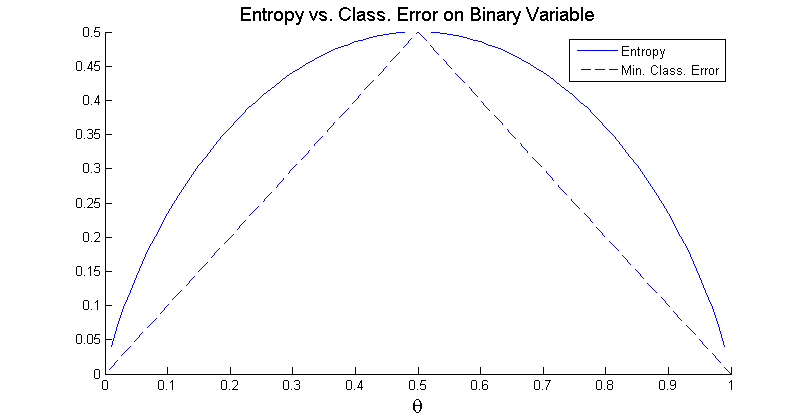
\includegraphics[scale=0.8]{assets/p1a3.png}
\end{center}
\subsection{Train a Decision Tree}
\begin{minipage}{0.5\linewidth}
	\begin{equation*}
	P(Y=y|X=x) = \frac{Count(Y=y,X=x)}{Count(X=x)}
	\end{equation*}
\end{minipage}
\begin{minipage}{0.5\linewidth}
	\begin{equation*}
	P(X=x_{1},Y=y_{1}) = \frac{Count(X=x_{1},Y=y_{1})}{\sum_{x\in X,y\in Y}Count(X=x,Y=y)}
	\end{equation*}
\end{minipage}

\begin{center}
\begin{minipage}{0.2\linewidth}
	\begin{tabular}{r| l}
	P(Y=Yes) & 0.32\\
	P(Y=No)  & 0.68\\
	\end{tabular}
\end{minipage}
\begin{minipage}{0.7\linewidth}
	\begin{tabular}{r| r r r r r r}
	 P(Y|X) & A=Child & A=Adult & C=First & C=Lower & G=Male & G=Female\\\hline
	 Y=Yes & 0.52 & 0.31 & 0.62 & 0.27 & 0.21 & 0.73\\
	 Y=No  & 0.48 & 0.69 & 0.38 & 0.73	& 0.79 & 0.27\\
	 \multicolumn{1}{!{\vrule width 0pt}c!{\vrule width 0pt}}{}\\
	 P(Y,X) & A=Child & A=Adult & C=First & C=Lower & G=Male & G=Female\\\hline
	 Y=Yes & 0.03 & 0.30 & 0.09 & 0.23 & 0.17 & 0.16\\
	 Y=No  & 0.02 & 0.65 & 0.06 & 0.62	& 0.62 & 0.06\\
	\end{tabular}
\end{minipage}
\end{center}

\begin{align*}
H(Y)&=-\theta log_{e}(\theta)-(1-\theta)log_{e}(1-\theta)\\
&=(0.32)log_{e}(0.32)-(1-(0.32))log_{e}(1-(0.32))\\
&=0.63\\\\
I(A;Y) &= H(Y)-H(Y|A)\\
&=H(Y)+\sum_{a,y}p(a,y)log_{e}p(y|a)\\
&=0.63+[0.03log_{e}0.52+0.02log_{e}0.48+0.30log_{e}0.31+0.65log_{e}0.69]\\
&=0.003
\\\\
I(C;Y) &= H(Y)-H(Y|C)\\
&=H(Y)+\sum_{c,y}p(c,y)log_{e}p(y|c)\\
&=0.63+[0.09log_{e}0.62+0.06log_{e}0.38+0.23log_{e}0.27+0.62log_{e}0.73]\\
&=0.03
\\\\
I(G;Y) &= H(Y)-H(Y|G)\\
&=H(Y)+\sum_{g,y}p(g,y)log_{e}p(y|g)\\
&=0.63+[0.17log_{e}0.21+0.62log_{e}0.79+0.16log_{e}0.73+0.06log_{e}0.27]\\
&=0.09
\end{align*}
The feature with the highest information gain is gender.

\section*{Code}
\subsection*{Problem 1.A.3}
\lstinputlisting[language=Matlab]{assets/p1a3.m}
\end{document}
